% !TEX root = ./main.tex
% !TEX encoding = UTF-8 Unicode
% !TEX program = pdflatex
% !TeX spellcheck = it_IT

\graphicspath{{Immagini/},{Immagini/pca_clustering/}}

\chapter{PCA \& Clustering}
Estrapolare un Workload sintetico a partire dal workload reale, riportato nel file
 \textit{PCA-CLASTERING-2017.jmp}.

\section{Obiettivo}
A partire dal workload reale, si vuole ottenere un \textbf{workload sintetico},
caratterizzato da un numero di osservazioni minori, che conservi quanta
più varianza possibile.

\section{Estrazione del Workload Sintetico}
Per estrarre il workload sintetico, dopo aver visionato i dati, si è scelto
di seguire il seguente procedimento:

\begin{itemize}
  \item Analisi del \textbf{\textit{CV(Coefficiente di Variazione)}}, per
  eliminare i parametri statisticamente non significativi;
  \item \textbf{\textit{PCA(Principal Component Analysis)}}, per ridurre il
  numero di parametri ed eliminare la correlazione tra essi;
  \item \textbf{\textit{Clustering}}, per ridurre il numero di esperimenti.
\end{itemize}


\subsection{Analisi del Coefficiente di Variazione}
In prima istanza, è stata effettuata un'analisi sul coefficiente di variazione(CV),
il quale esprime la dispersione dei valori dei singoli parametri attorno alla loro media.\\
Quando il coefficiente di variazione è nullo, il parametro
corrispondente non è statisticamente significativo e quindi è possibile eliminarlo.\\
Nella \figurename~\ref{cv} si evince l'assenza di colonne con coefficiente di variazione nullo,
quindi tutti i parametri dovranno essere utilizzati nelle successive fasi di analisi.

\begin{figure}[!htbp]
  \centering
	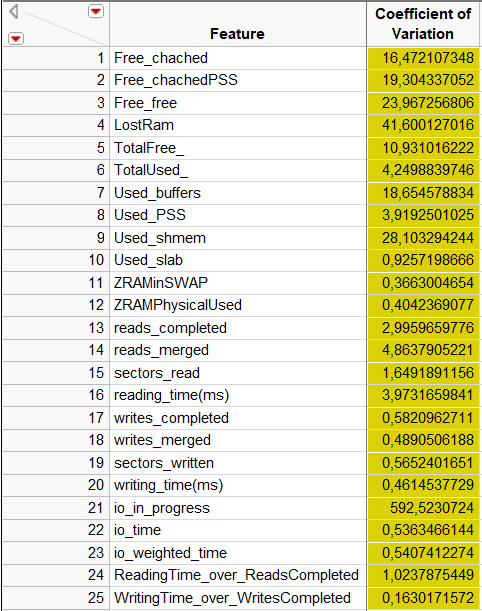
\includegraphics[width=.7\linewidth,keepaspectratio]{cov.png}
  \caption{Coefficiente di Variazione(CV)}
  \label{cv}
\end{figure}
\clearpage

\subsection{PCA}
In questa fase è stata applicata la
\textbf{\textit{PCA(Principal Component Analysis)}},
la quale trasforma un workload con parametri correlati in uno contenente parametri
incorrelati, ottenuti come combinazione lineare, pesata, di quelli iniziali.\\
L'utilizzo della PCA è fondamentale anche per la successiva fase di clustering, in
quanto quest'ultimo necessita che sia rispettata la proprietà di incorrelazione
dei parametri.\\
Per effettuare la PCA si è fatto utilizzo del tool statistico \textit{\textbf{JMP}}, nella
\figurename~\ref{pca} è riportato l'output.\\

\begin{figure}[!htbp]
	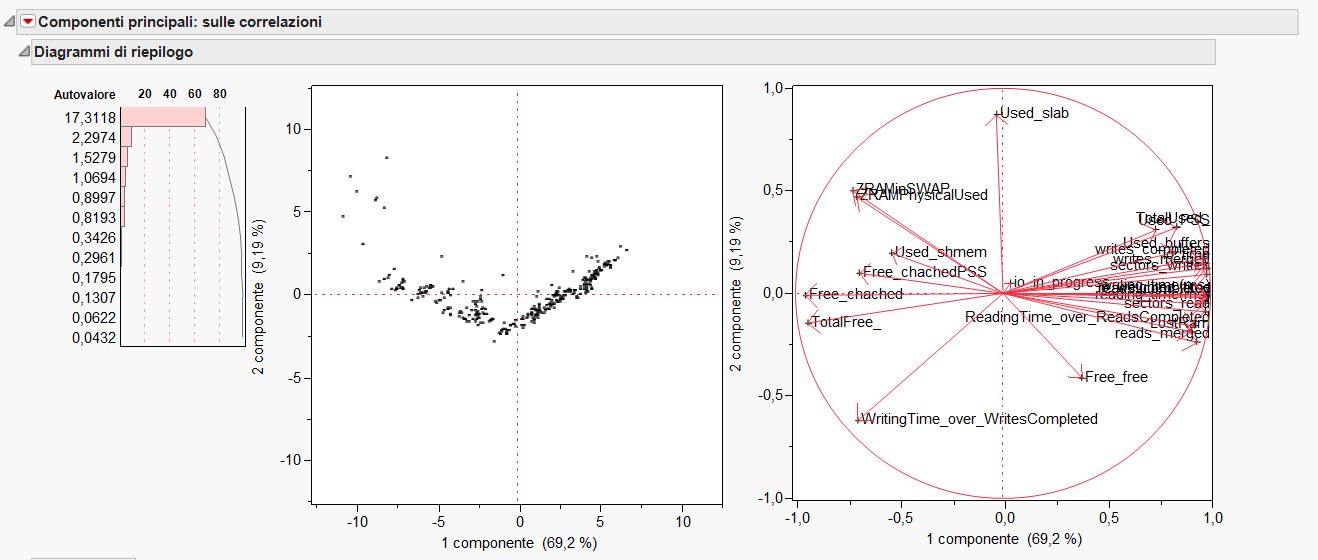
\includegraphics[width=\linewidth,keepaspectratio]{pca.png}
  \caption{Risultato PCA}
  \label{pca}
\end{figure}

\clearpage

Nella \figurename~\ref{autovalori} sono riportati gli autovalori ottenuti dalla PCA.\\

\begin{figure}[!htbp]
	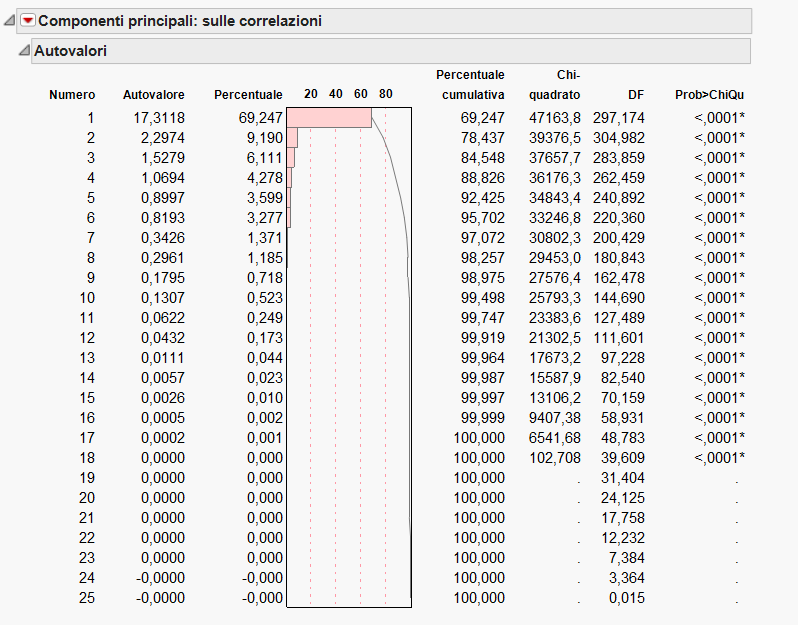
\includegraphics[width=\linewidth,keepaspectratio]{autovalori.png}
  \caption{Autovalori PCA}
  \label{autovalori}
\end{figure}

\clearpage

\begin{figure}[!htbp]
	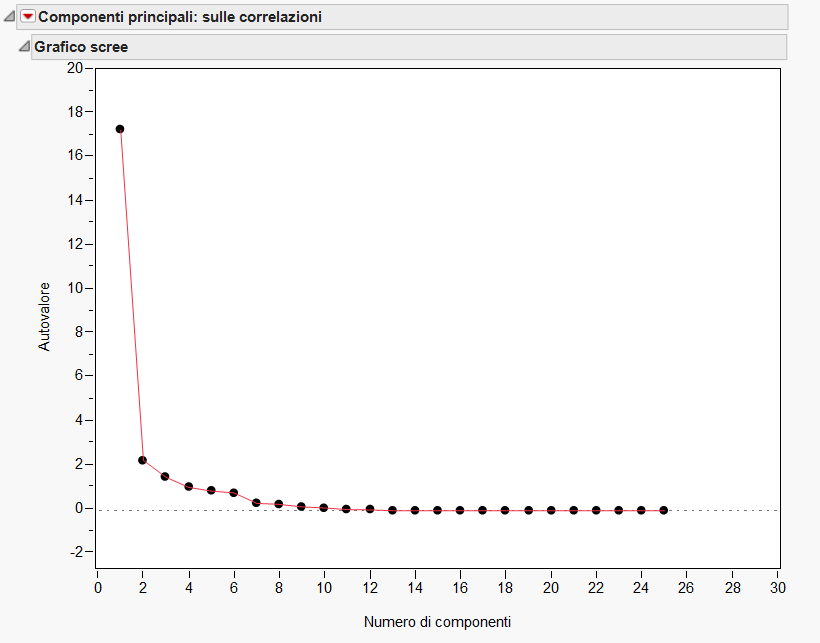
\includegraphics[width=\linewidth,keepaspectratio]{grafico_scree.png}
  \caption{Grafico Scree}
  \label{grafico_scree}
\end{figure}

\'E possibile scegliere il numero di componenti principali da utilizzare considerando
il ginocchio della curva ottenuta nella \figurename~\ref{grafico_scree}, rappresentante
sull'asse x il numero di componenti principali e sull'asse y
gli autovalori.\\
In questo caso, scegliendo di considerare 6 componenti principali, si è sicuri di conservare una quota di varianza sufficientemente
significativa(\textit{95,703\%}).\\
\clearpage
\begin{figure}[!htbp]
	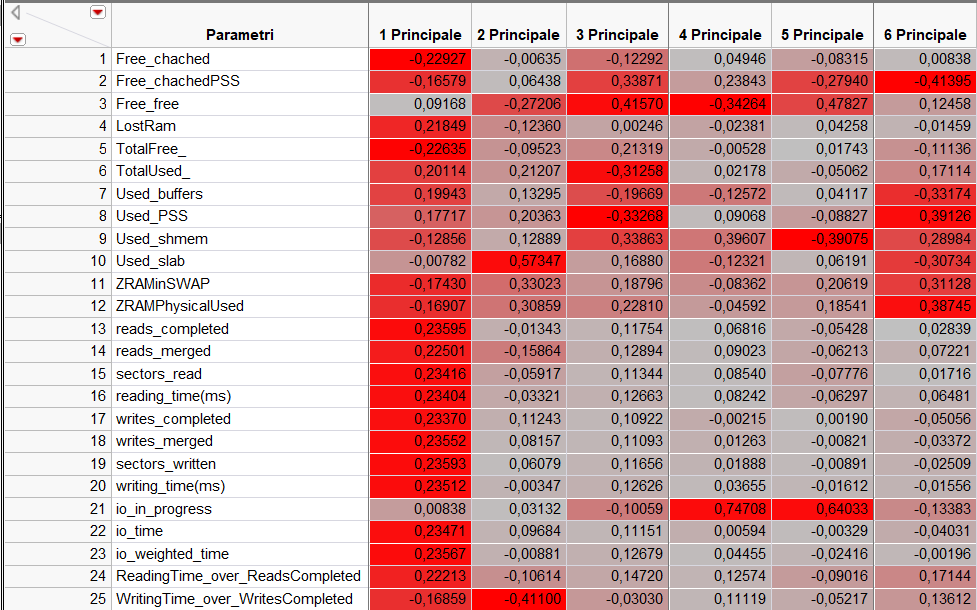
\includegraphics[width=\linewidth,keepaspectratio]{autovettori.png}
  \caption{Autovettori}
  \label{autovettori}
\end{figure}

Nella \figurename~\ref{autovettori} sono sfumati in rosso i parametri che
hanno contribuito maggiormente, in segno positivo o negativo, alla creazione
delle componenti principali scelte.\\
Valori vicini allo 0 indicano che quei parametri pesano relativamente poco nel
calcolo della componente principale.\\

% In particolare:
% \begin{itemize}
%   \item \textbf{\textit{Principale 1:}} \textit{Free\_chached, LostRam, TotalFree,
%   reads\_completed, reads\_merged, sectors\_read, reading\_time(ms),
%   writes\_completed, writes\_merged, sector\_written, writing\_time(ms),
%   io\_time, io\_weighted\_time e ReadingTime\_over\_ReadsCompleted};
%   \item \textbf{\textit{Principale 2:}} \textit{Used\_slab e WritingTime\_over\_WritesCompleted};
%   \item \textbf{\textit{Principale 3:}} \textit{Free\_free, TotalUsed e Used\_PSS};
%   \item \textbf{\textit{Principale 4:}} \textit{io\_in\_progress};
%   \item \textbf{\textit{Principale 5:}} \textit{Used\_shmem};autovettori
%   \item \textbf{\textit{Principale 6:}} \textit{Free\_chachedPSS, Used\_buffers e Used\_PSS, ZRamPhysicalUsed};
% \end{itemize}
\clearpage
\subsection{Clustering}
In questa fase è stato effettuata un'operazione di clustering sul risultato
ottenuto dallo step precedente.\\
La tecnica di clusterizzazione scelta è di tipo gerarchico agglomerativo,
in particolare è stata utilizzata la metrica di \textbf{Ward} per l'aggregazione
dei cluster.\\
Il criterio di Ward è diretto alla minimizzazione della varianza all’interno dei gruppi,
pertanto si presta bene ad essere utilizzato con variabili quantitative.\\
In \figurename~\ref{dendrogramma} è riportato il dendrogramma risultante.\\

\begin{figure}[!htbp]
	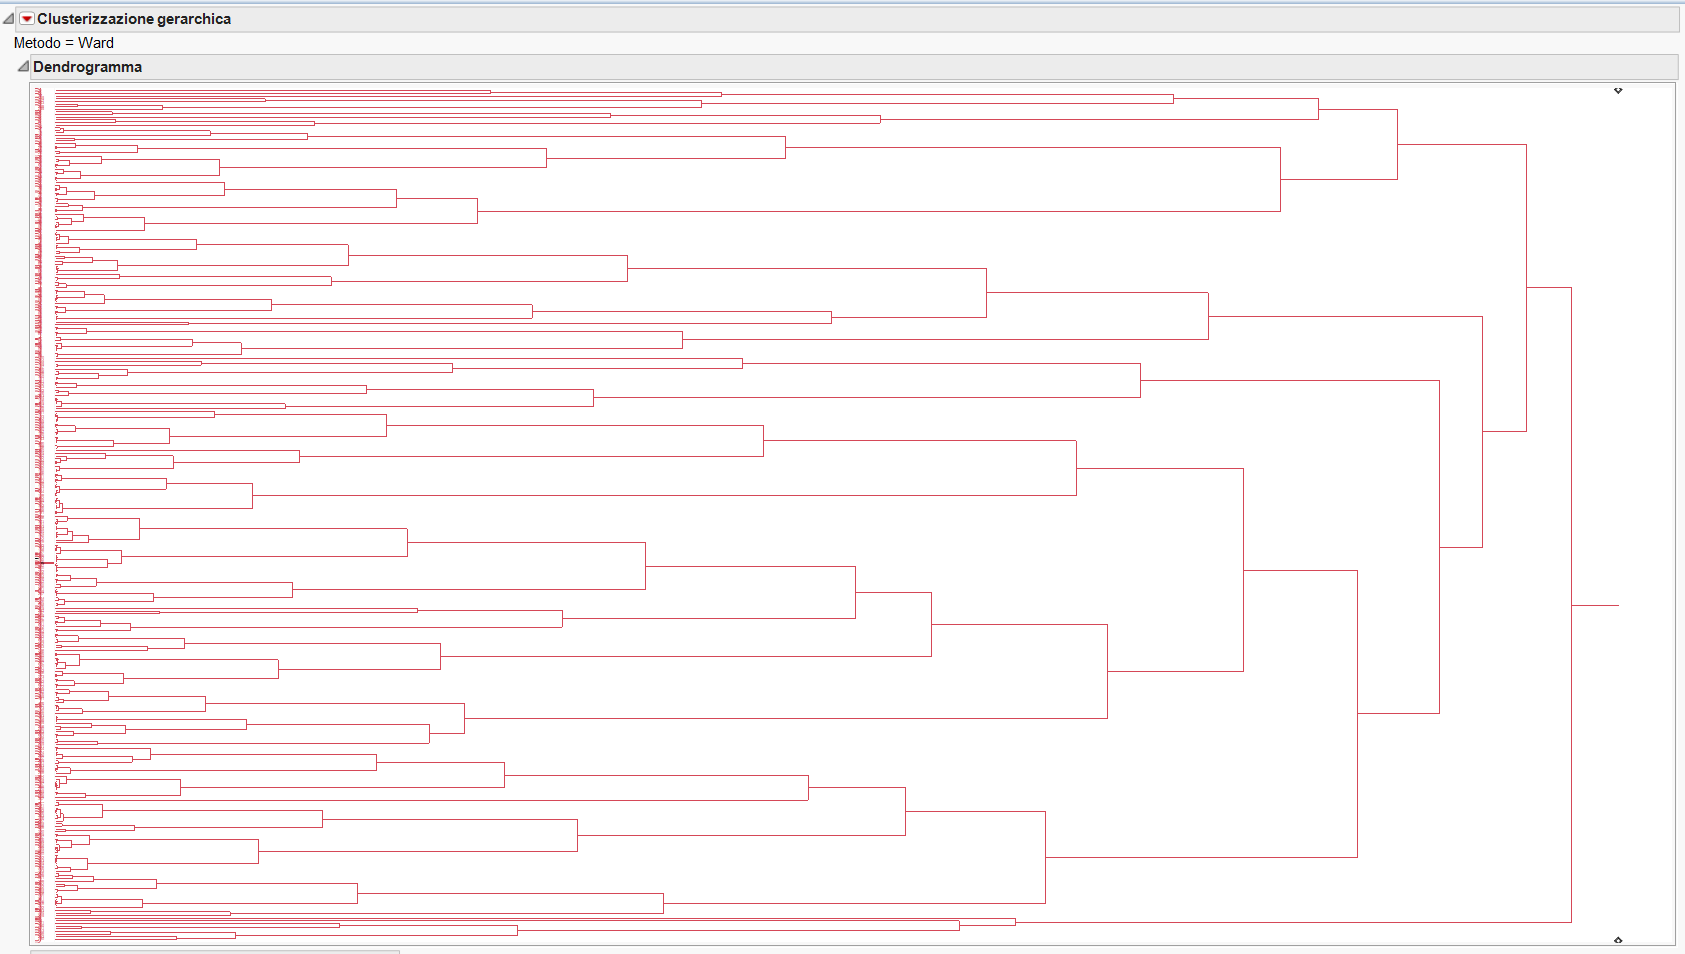
\includegraphics[width=\linewidth,keepaspectratio]{dendrogramma.png}
  \caption{Dendrogramma}
  \label{dendrogramma}
\end{figure}
\clearpage
\begin{figure}[!htbp]
	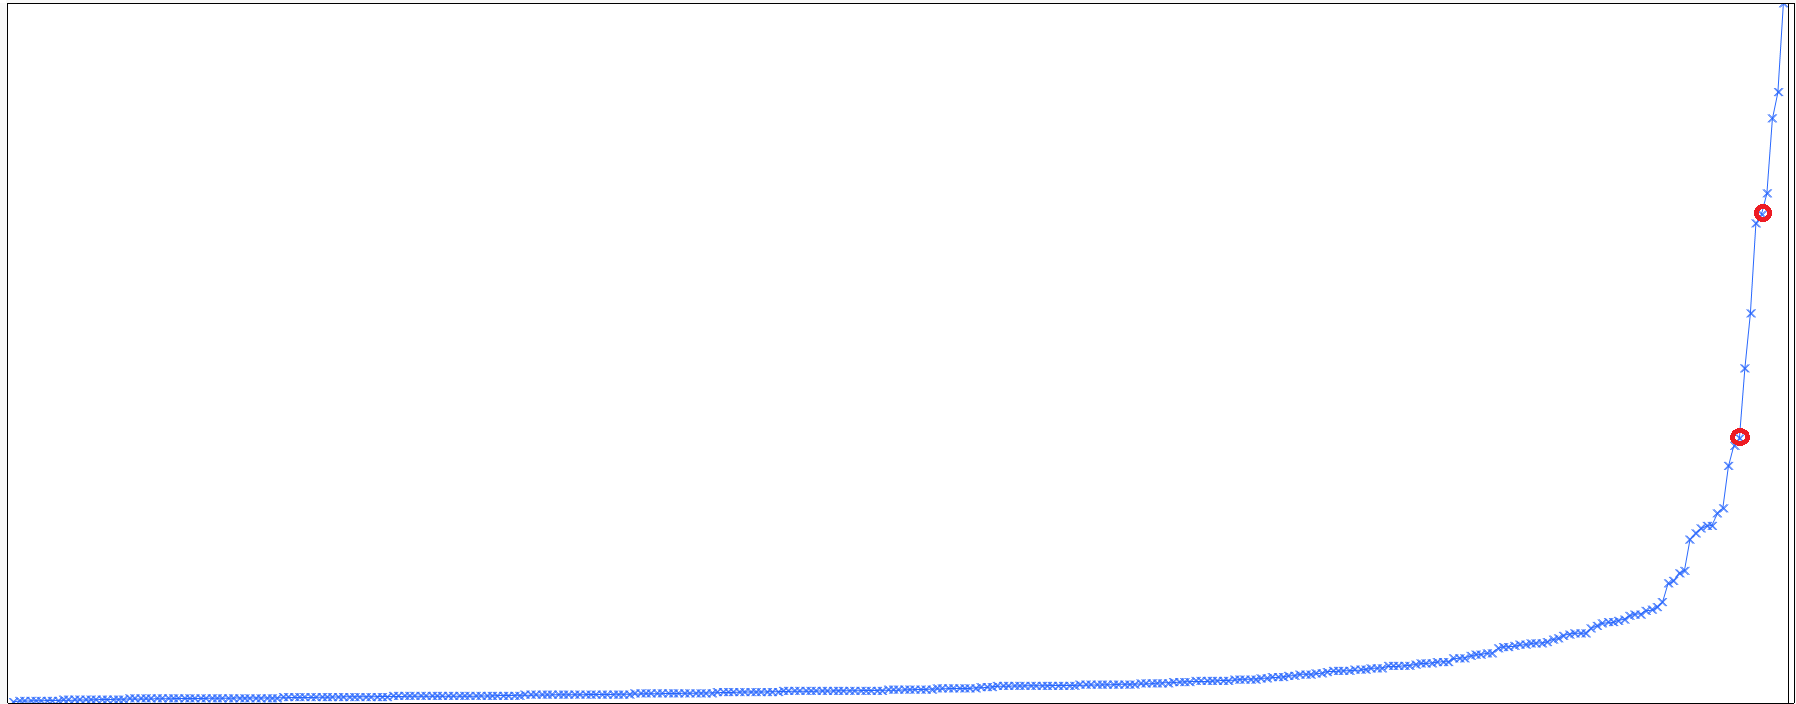
\includegraphics[width=\linewidth,keepaspectratio]{curva_dendrogramma.png}
  \caption{Curva di Clustering}
  \label{curva_dendrogramma}
\end{figure}

Facendo riferimento alla \figurename~\ref{curva_dendrogramma}, è possibile scegliere
il numero di cluster posizionandosi nel ginocchio della curva, rappresentante le
distanze tra cluster.\\
In maniera analoga si può scegliere il numero di cluster utilizzando il criterio
di clusterizzazione cubica(\textbf{CCC}), riportato in \figurename~\ref{ccc},
scegliendo il numero di cluster in funzione della regola del massimo salto.\\

\begin{figure}[htbp]
\centering
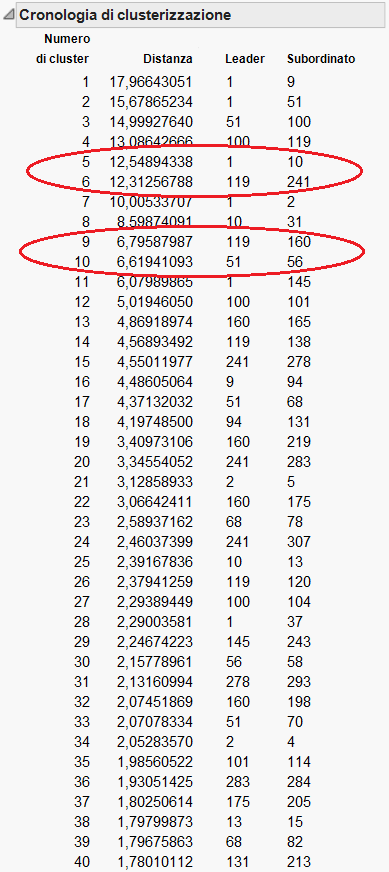
\includegraphics[width=50mm]{gerarchia_clustering.png}% "%" necessario
\qquad\qquad
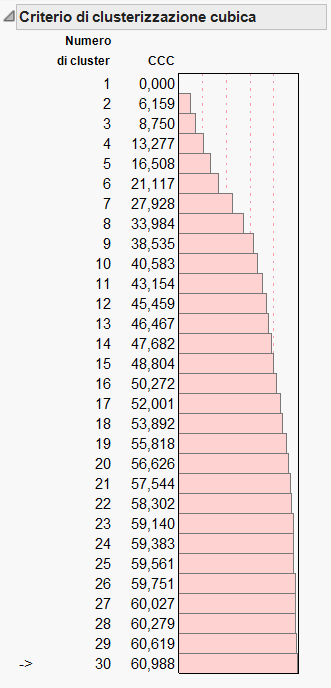
\includegraphics[width=50mm]{ccc.png}
\caption{Gerarchia Clustering e Criterio di Clusterizzazione Cubica}
\label{ccc}
\end{figure}

\clearpage

Sulla base dei criteri illustrati, si è scelto di considerare due soluzioni:
5 e 9 cluster.\\
Per generare i workload sintetici, inoltre, si è scelto di considerare il
centroide di ogni cluster.\\

\begin{figure}[!htbp]
	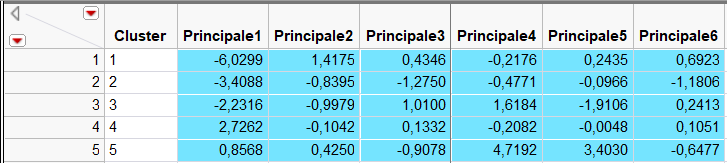
\includegraphics[width=\linewidth,keepaspectratio]{centroidi(5).png}
  \caption{Workload sintetico ottenuto con 5 cluster}
  \label{}
\end{figure}

\begin{figure}[!htbp]
	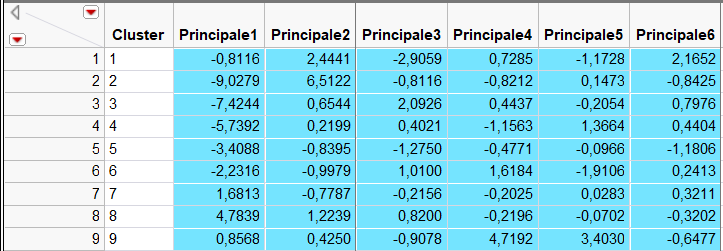
\includegraphics[width=\linewidth,keepaspectratio]{centroidi(9).png}
  \caption{Workload sintetico ottenuto con 9 cluster}
  \label{centroidi9}
\end{figure}

\clearpage
\section{Analisi}
Ottenuti i Workload Sintetici, è fondamentale osservare quanta varianza si è
conservata.\\
Per capire se la soluzione a 9 cluster è più conveniente della soluzione
a 5 cluster, bisogna confrontare la significatività conservata dai due workload sintetici.\\
Per fare ciò bisogna calcolare la varianza persa in ogni fase del processo di
caratterizzazione.\\
A valle della PCA, scegliendo solo 6 componenti principali, la varianza conservata
 risulta essere il 95,702\% della totale(valore ottenuto in JMP).\\
Per definire la significatività dei workload ottenuti con il clustering, invece, bisogna
utilizzare la devianza.\\
Quest'ultima è una grandezza indipendente dal grado di libertà, quindi si presta
perfettamente all'uso con i cluster, i quali hanno cardinalità differente.\\

La devianza del clustering è calcolata come la somma della devianza \textbf{inter-cluster}
e \textbf{intra-cluster}.\\
Tipicamente, per effettuare un buon clustering, si cerca di massimizzare la varianza
inter-clustering e minimizzare quella intra-clustering.\\
Nella seguente figura è riportata la devianza del workload sottoposto a PCA.\\

\begin{figure}[!htbp]
  \centering
	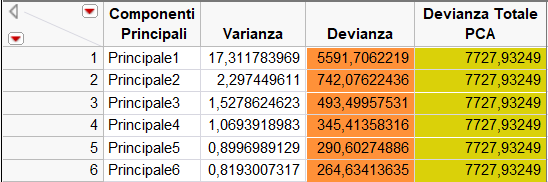
\includegraphics[width=.7\linewidth,keepaspectratio]{devianza_pca.png}
  \caption{Devianza PCA}
  \label{}
\end{figure}
\clearpage

\subsubsection{5 cluster}

Nella seguente figura è riportata la devianza inter-cluster.\\

\begin{figure}[!htbp]
  \centering
	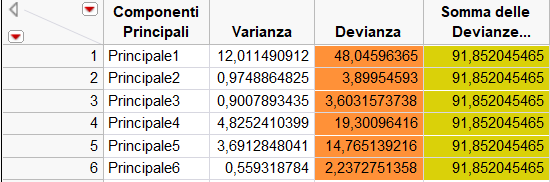
\includegraphics[width=.7\linewidth,keepaspectratio]{devianza_inter_clusters(5).png}
  \caption{Devianza Inter-Cluster}
  \label{}
\end{figure}

Nella seguente figura è riportata la devianza intra-cluster.\\

\begin{figure}[!htbp]
  \centering
	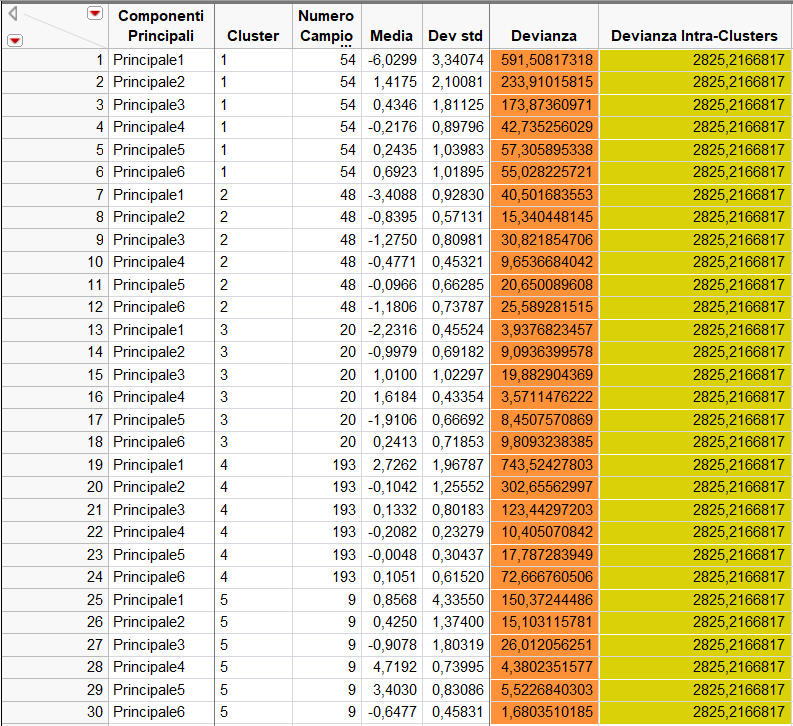
\includegraphics[width=.7\linewidth,keepaspectratio]{devianza_intra_clusters(5).png}
  \caption{Devianza Intra-Cluster}
  \label{}
\end{figure}
\clearpage

\subsubsection{9 cluster}

Nella seguente figura è riportata la devianza inter-cluster.\\

\begin{figure}[!htbp]
  \centering
	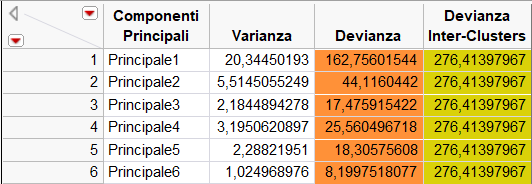
\includegraphics[width=.7\linewidth,keepaspectratio]{devianza_inter_clusters(9).png}
  \caption{Devianza Inter-Cluster}
  \label{}
\end{figure}

Nella seguente figura è riportata la devianza intra-cluster.\\

\begin{figure}[!htbp]
  \centering
	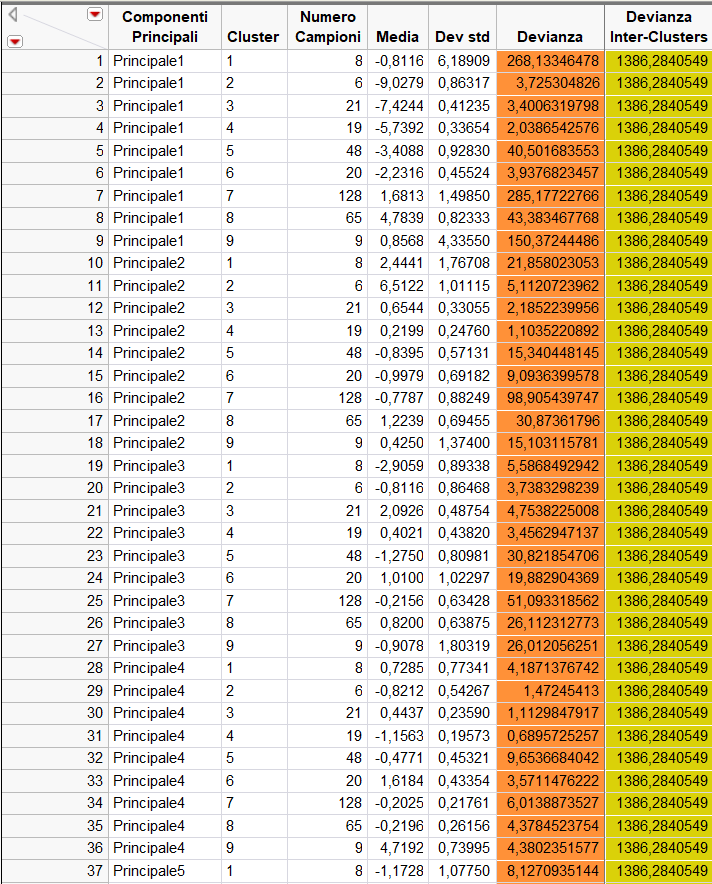
\includegraphics[width=.5\linewidth,keepaspectratio]{devianza_intra_clusters(9).png}
  \caption{Devianza Intra-Cluster}
  \label{}
\end{figure}
\clearpage
\section{Conclusioni}

Dopo aver ottenuto i valori di devianza del workload sottoposto a PCA e, successivamente,
a Clustering, considerando 5 e 9 cluster, è possibile calcolarne la significatività.\\
La devianza conservata utilizzando la tecnica di clustering si calcola con la
seguente formula:
$$1-{devianza_{inter\_cluster}+devianza_{intra\_cluster}\over {devianza_{pca}}}$$

Nelle seguenti Tabelle sono riportate le percentuali di devianza persa e conservata,
 nei due casi analizzati.\\
\vspace{5 mm}

\begin{center}
  \textbf{5 Cluster}
\end{center}
\begin{figure}[!htbp]
  \centering
  \begin{tabular}{|c|c|}
  \hline
  \textbf{Devianza PCA}	& 7727,93249 \\
  \hline
  \textbf{Devianza Clustering(intra-cluster+inter-cluster)}	& 2917,0687 \\
  \hline
  \textbf{Percentuale devianza persa con il clustering}	& 37,75\% \\
  \hline
  \textbf{Percentuale devianza conservata con il clustering}	& 62,25\% \\
  \hline
  \textbf{Significatività PCA} &	95,70\% \\
  \hline
  \end{tabular}
  %\caption{Workload con 5 cluster}
\end{figure}


\vspace{5 mm}
\begin{center}
  \textbf{9 Cluster}
\end{center}
\begin{figure}[!htbp]
  \centering
  \begin{tabular}{|c|c|}
    \hline
    \textbf{Devianza PCA}	& 7727,93249 \\
    \hline
    \textbf{Devianza Clustering(intra-cluster+inter-cluster)}	& 1662,6980 \\
    \hline
    \textbf{Percentuale devianza persa con il clustering}	& 21,52\% \\
    \hline
    \textbf{Percentuale devianza conservata con il clustering}	& 78,48\% \\
    \hline
    \textbf{Significatività PCA} &	95,70\% \\
    \hline
  \end{tabular}
  %\caption{Workload con 9 cluster}
\end{figure}

\clearpage

In seguito sono riportate le tabelle che riassumono la significatività perduta e
conservata a partire dal Workload Reale fino a quello Sintetico, ottenuto con
PCA e Clustering.\\

\vspace{5 mm}
\begin{center}
  \textbf{5 Cluster}
\end{center}
\begin{figure}[!htbp]
  \centering
  \begin{tabular}{c|c|c}
   & \textbf{Conservata} & \textbf{Perse} \\
   \hline
   \textbf{Workload Reale} & 100,00\% &	0,00\% \\
   \hline
   \textbf{PCA} &	95,70\%	& 4,30\% \\
   \hline
   \textbf{Clustering} &	59,58\%	& 40,42\% \\
  \end{tabular}
  % \caption{Significatività Workload con 5 cluster}
\end{figure}

\vspace{5 mm}
\begin{center}
  \textbf{9 Cluster}
\end{center}
\begin{figure}[!htbp]
  \centering
  \begin{tabular}{c|c|c}
   & \textbf{Conservata} & \textbf{Persa} \\
   \hline
   \textbf{Workload Reale} & 100,00\% &	0,00\% \\
   \hline
   \textbf{PCA} &	95,70\%	& 4,30\% \\
   \hline
   \textbf{Clustering} &	75,11\%	& 24,89\% \\
  \end{tabular}
  % \caption{Significatività Workload con 9 cluster}
\end{figure}

\vspace{5 mm}

In conclusione, utilizzando 6 componenti principali e 5 cluster, si perde il 40,42\%
di significatività rispetto al workload reale mentre scegliendo 9 cluster si perde il 24,89\%.\\
La percentuale di varianza conservata considerando 9 cluster è notevolmente maggiore,
con il compromesso di dover effettuare 9 esperimenti.\\
Quindi si può affermare che, se non ci sono particolari limitazioni di costo e/o tempo,
il workload sintetico con 9 cluster rappresenta una soluzione migliore.\\
Per sottoporre il Workload Sintetico al sistema da testare è necessario identificare
quali sono i parametri del Workload Reale che contribuiscono maggiormente
alla formazione delle componenti principali utilizzate.\\
Tale operazione si effettua considerando la matrice degli autovettori, riportata
in \figurename~\ref{autovettori}, e scegliendo solo i quattro parametri con maggior
peso, due negativi e due positivi, per ogni PC.\\
Successivamente, in accordo con il segno del valori rispetto ad ogni componente
principale, presenti in \figurename~\ref{centroidi9}, si caratterizzano i
differenti cluster o con i due parametri positivi scelti o con i due negativi.\\
In tabella è riportato il risultato ottenuto.
\begin{figure}
\centering
   \begin{tabular}{p{0.1\linewidth} || p{0.4\linewidth} | p{0.55\linewidth}}
     \textbf{Cluster} & \textbf{Principale 1} & \textbf{Principale 2} \\
     \hline
     \hline
     \textbf{1} & \textit{Free\_cached, TotalFree\_} & \textit{Used\_slab, ZRAMinSWAP} \\
     \hline
     \textbf{2} & \textit{Free\_cached, TotalFree\_} & \textit{Used\_slab, ZRAMinSWAP} \\
     \hline
     \textbf{3} & \textit{Free\_cached, TotalFree\_} & \textit{Used\_slab, ZRAMinSWAP} \\
     \hline
     \textbf{4} & \textit{Free\_cached, TotalFree\_} & \textit{Used\_slab, ZRAMinSWAP} \\
     \hline
     \textbf{5} & \textit{Free\_cached, TotalFree\_} & \textit{WritingTime\_over\_WritesCompleted, Free\_free} \\
     \hline
     \textbf{6} & \textit{Free\_cached, TotalFree\_} & \textit{WritingTime\_over\_WritesCompleted, Free\_free} \\
     \hline
     \textbf{7} & \textit{reads\_completed, sectors\_written} &	\textit{WritingTime\_over\_WritesCompleted, Free\_free} \\
     \hline
     \textbf{8} &  \textit{reads\_completed, sectors\_written} & \textit{Used\_slab, ZRAMinSWAP} \\
     \hline
     \textbf{9} &  \textit{reads\_completed, sectors\_written} & \textit{Used\_slab, ZRAMinSWAP} \\
     \hline
   \end{tabular}
  \begin{tabular}{p{0.1\linewidth} || p{0.4\linewidth} | p{0.55\linewidth}}
   & \textbf{Principale 3} & \textbf{Principale 4}  \\
    \hline
    \hline
    \textbf{1} & \textit{Used\_PSS, TotalUsed\_} & \textit{io\_in\_progress, Used\_shmem} \\
    \hline
    \textbf{2} & \textit{Used\_PSS, TotalUsed\_} & \textit{Free\_free, Used\_buffers} \\
    \hline
    \textbf{3} & \textit{Free\_free, Free\_chachedPSS} & \textit{io\_in\_progress, Used\_shmem} \\
    \hline
    \textbf{4} & \textit{Free\_free, Free\_chachedPSS} & \textit{Free\_free, Used\_buffers} \\
    \hline
    \textbf{5} & \textit{Used\_PSS, TotalUsed\_}  & \textit{Free\_free, Used\_buffers} \\
    \hline
    \textbf{6} & \textit{Free\_free, Free\_chachedPSS} & \textit{io\_in\_progress, Used\_shmem} \\
    \hline
    \textbf{7} & \textit{Used\_PSS, TotalUsed\_}  & \textit{Free\_free, Used\_buffers} \\
    \hline
    \textbf{8} & \textit{Free\_free, Free\_chachedPSS} & \textit{Free\_free, Used\_buffers} \\
    \hline
    \textbf{9} & \textit{Used\_PSS, TotalUsed\_} & \textit{io\_in\_progress, Used\_shmem} \\
    \hline
  \end{tabular}
  \begin{tabular}{p{0.1\linewidth} || p{0.4\linewidth} | p{0.55\linewidth}}
    & \textbf{Principale 5} & \textbf{Principale 6}  \\
   \hline
   \hline
   \textbf{1} & \textit{Used\_shmem, Free\_chachedPSS} & \textit{Used\_PSS, ZRAMPhysicalUsed} \\
   \hline
   \textbf{2} & \textit{io\_in\_progress, Free\_free} & \textit{Free\_chachedPSS, Used\_buffers} \\
   \hline
   \textbf{3} & \textit{Used\_shmem, Free\_chachedPSS} & \textit{Used\_PSS, ZRAMPhysicalUsed} \\
   \hline
   \textbf{4} & \textit{io\_in\_progress, Free\_free} & \textit{Used\_PSS, ZRAMPhysicalUsed} \\
   \hline
   \textbf{5} & \textit{Used\_shmem, Free\_chachedPSS} & \textit{Free\_chachedPSS, Used\_buffers} \\
   \hline
   \textbf{6} & \textit{Used\_shmem, Free\_chachedPSS} & \textit{Used\_PSS, ZRAMPhysicalUsed} \\
   \hline
   \textbf{7} & \textit{io\_in\_progress, Free\_free} & \textit{Used\_PSS, ZRAMPhysicalUsed} \\
   \hline
   \textbf{8} & \textit{Used\_shmem, Free\_chachedPSS} & \textit{Free\_chachedPSS, Used\_buffers} \\
   \hline
   \textbf{9} & \textit{io\_in\_progress, Free\_free} & \textit{Free\_chachedPSS, Used\_buffers} \\
   \hline
  \end{tabular}
  \caption{Parametri Caratterizzanti il Workload Sintetico con 9 cluster}
  \end{figure}
